\begin{figure}[t]
\centering
\setlength{\tabcolsep}{4pt}
\begin{tabular}{@{}cc@{}}
\footnotesize\textbf{(a) Easy: easy-0001, 4 folds} &
\footnotesize\textbf{(b) Medium: mid-0004, 11 folds}\\[2pt]
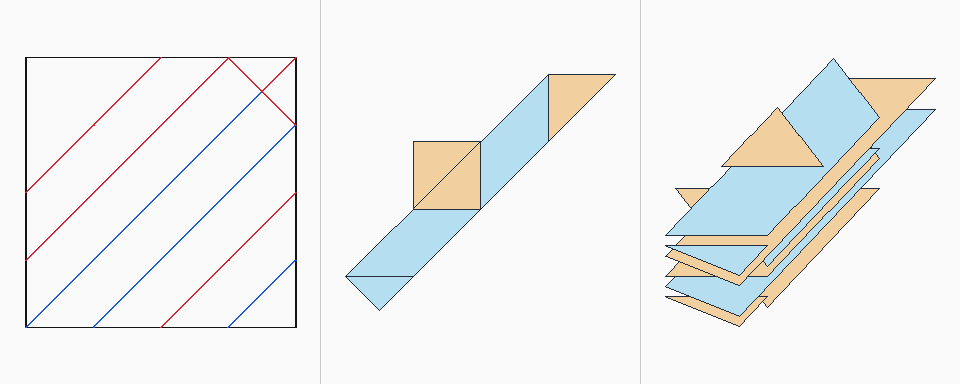
\includegraphics[width=.47\linewidth,trim=0 0 320bp 0,clip]{figures/dataset/sample-1.png}&
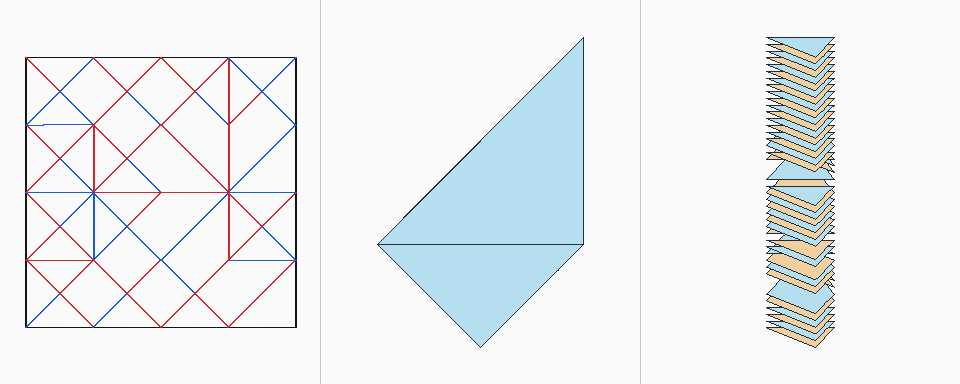
\includegraphics[width=.47\linewidth,trim=0 0 320bp 0,clip]{figures/dataset/sample-2.png}\\[5pt]
\footnotesize\textbf{(c) Hard: hard-0004, 15 folds} &
\footnotesize\textbf{(d) Some-layers: layers-0001, 5 folds}\\[2pt]
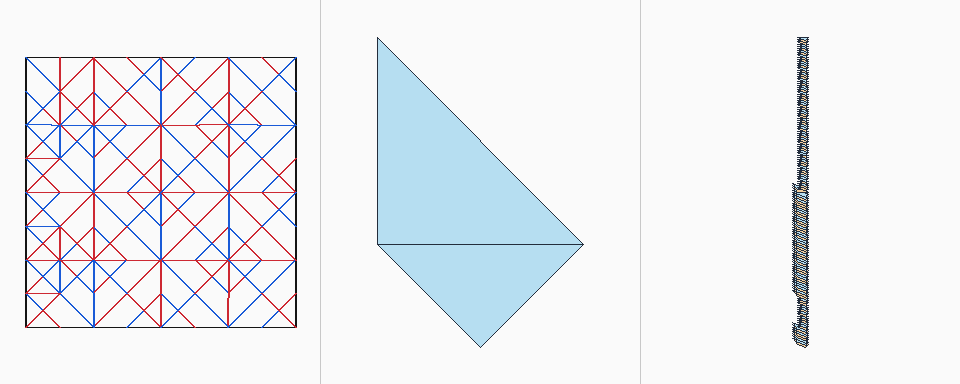
\includegraphics[width=.47\linewidth,trim=0 0 320bp 0,clip]{figures/dataset/sample-4.png}&
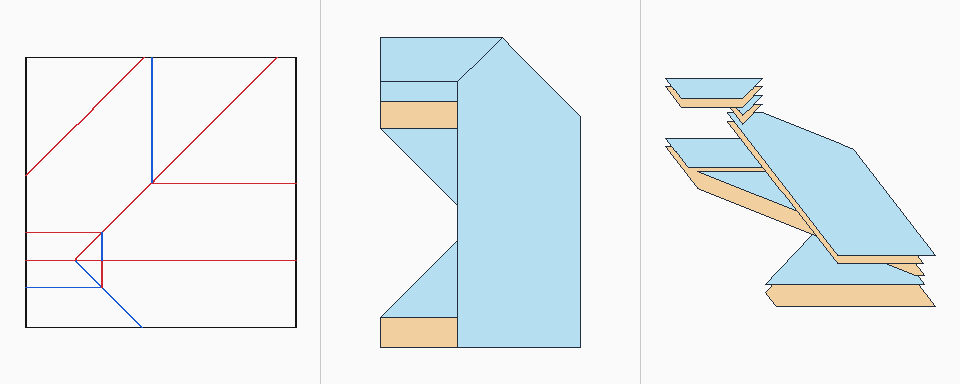
\includegraphics[width=.47\linewidth,trim=0 0 320bp 0,clip]{figures/dataset/sample-3.png}
\end{tabular}
\caption{CP2Seq examples: each panel pairs the crease pattern (left) with the target top view
(right). Panels (a--c) use all-layers folds; (d) is from some-generated-d5. Counts are reference
folds. Red and blue denote mountain and valley creases.}
\label{fig:dataset-examples}
\end{figure}
